\documentclass[tikz,border=2pt]{standalone}
\usepackage{amsmath}
\usetikzlibrary{arrows.meta}
\begin{document}
% Round trip of a small table: the text file (header + 3 lines) -> read.csv() -> data frame;
% write.csv(..., row.names = FALSE) writes it back to the working directory.
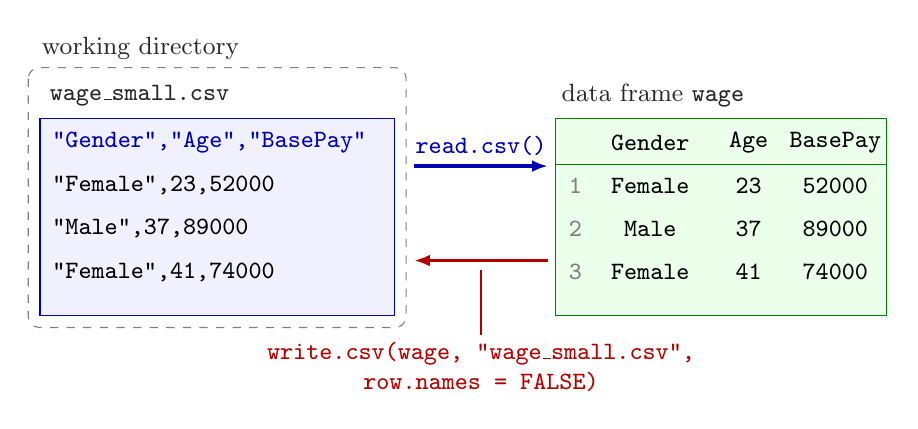
\begin{tikzpicture}[font=\small, >={Latex[length=2mm]},
  txt/.style={anchor=west, inner sep=0pt, font=\small\ttfamily},
  hd/.style={font=\small\ttfamily\bfseries}]
  % working directory and file
  \draw[gray, dashed, rounded corners=4pt] (-0.35,0.95) rectangle (4.45,-2.35);
  \node[anchor=west, gray!30!black] at (-0.3,1.2) {working directory};
  \node[anchor=west, font=\small\ttfamily, gray!30!black] at (-0.2,0.6) {wage\_small.csv};
  \draw[blue!70!black, fill=blue!6] (-0.2,0.3) rectangle (4.3,-2.2);
  \node[txt, blue!70!black] at (-0.05,0.0)  {"Gender","Age","BasePay"};
  \node[txt] at (-0.05,-0.55) {"Female",23,52000};
  \node[txt] at (-0.05,-1.1)  {"Male",37,89000};
  \node[txt] at (-0.05,-1.65) {"Female",41,74000};
  % data frame
  \begin{scope}[xshift=6.6cm]
    \node[anchor=west, gray!30!black] at (-0.3,0.6) {data frame \texttt{wage}};
    \draw[green!50!black, fill=green!8] (-0.25,0.3) rectangle (3.95,-2.2);
    \draw[green!50!black] (-0.25,-0.28) -- (3.95,-0.28);
    \node[hd] at (0.95,0.0) {Gender}; \node[hd] at (2.2,0.0) {Age}; \node[hd] at (3.3,0.0) {BasePay};
    \foreach \r/\g/\a/\b [count=\i] in {1/Female/23/52000, 2/Male/37/89000, 3/Female/41/74000} {
      \node[gray, font=\small\ttfamily] at (0.0,-0.55*\i) {\r};
      \node[font=\small\ttfamily] at (0.95,-0.55*\i) {\g};
      \node[font=\small\ttfamily] at (2.2,-0.55*\i) {\a};
      \node[font=\small\ttfamily] at (3.3,-0.55*\i) {\b};
    }
  \end{scope}
  % arrows
  \draw[->, very thick, blue!70!black] (4.55,-0.3) -- node[above, font=\small\ttfamily] {read.csv()} (6.25,-0.3);
  \draw[<-, very thick, red!70!black] (4.55,-1.5) -- (6.25,-1.5);
  \node[red!70!black, font=\small\ttfamily, align=center] at (5.4,-2.85) {write.csv(wage, "wage\_small.csv",\\ row.names = FALSE)};
  \draw[red!70!black, thin] (5.4,-1.62) -- (5.4,-2.45);
\end{tikzpicture}
\end{document}
